
% This is a simple template for a LaTeX document using the "article" class.
% See "book", "report", "letter" for other types of document.

\documentclass[10pt]{article} % use larger type; default would be 10pt

\input{preamble.tex}

\begin{document}

% \vspace{-10pt}
% This is the PERFECT SCALING, now we need to adjust the scale a little bit.
\begin{tikzpicture}[remember picture,overlay,yshift=-.2cm, xshift=1.75cm] % LMAOOOOOO This is the EXACT POSITION!!!!
    \node at (0,0) {\includegraphics[width=4.0cm,height=1.6cm]{media/1280px-Logo_Polytech_Sorbonne.png}};
\end{tikzpicture}

% \hspace{-5cm}
% \hspace{-1cm}
% \hspace{-1cm}

\vspace{-1cm}
\vspace{0.3cm}

{\raggedleft \color{mygold} Algorithmique générale\\
MAIN-3, année 2022\\
Séance TP N\degree 3\\
Mars 2022\\
VOYLES Evan\\}

% This vspace accomodates my name
\vspace{-0.42cm}
\vspace{1.23cm}

{\Large \noindent \color{mygold} Objectif}

{\color{mygold}\noindent\rule{\textwidth}{1pt}}
\vspace{0cm}
\begin{itemize}
    \item[{\color{mygold}\ding{43}}] Arbres binaires de recherche.
\end{itemize}

\vspace{1.2cm}
{\color{dullgreen}\noindent \Large \bf Problème}

\vspace{-0.28cm}
{\vspace{0cm}\color{dullgreen}\noindent\rule{\textwidth}{1pt}}

\begin{textblock*}{8.75cm}(10.16cm,7.2cm) % {block width} (coords)
    \Large \aspurp{[Arbres binaires de recherce aléatoires]}
\end{textblock*}

\vspace{1cm}

La documentation générale pour ce travail se trouve \href{https://polytech-sorbonne-main-tp2.readthedocs.io/en/latest/}{ici}, la documentation
technique se trouve \href{https://ejovo13.github.io/DSA_TP1/}{là}, et \href{https://github.com/ejovo13/DSA_TP1}{voici} le répertoire git.

\vspace{1cm}
\noindent \asgold{Partie A :} \aspurp{Structure Abr}

La structure \texttt{bin\_tree\_t} et toutes les fonctions définies autour cet objet encodent l'interface pour un arbre
binaire de recherche.

\begin{itemize}
    % \item Réaliser un suivi à la trace de la procédure \verb|partitionBis| appliquée aux instances suivantes :
    \item[\ding{43}] l'insertion d'une nouvelle clé dans l'arbre.
\end{itemize}

% /* #include "tree.h" */
\begin{lstlisting}[language=C, keywordstyle=\color{objectPurp}, otherkeywords={root}]
    // Instantiation
    BinTree *root = newBinTree(10);

    // insertion
    |\color{functionColor}addKeyBST|(root, 1);
    |\color{functionColor}addKeyBST|(root, 0);
    |\color{functionColor}addKeyBST|(root, 13);
    |\color{functionColor}addKeyBST|(root, 5);
    |\color{functionColor}addKeyBST|(root, 8);
    |\color{functionColor}addKeyBST|(root, 25);
    |\color{functionColor}addKeyBST|(root, 3);
\end{lstlisting}

Cet extrait de code encode l'arbre suivant (obtenu après un appel à la fonction \texttt{createDotBST}) :

\begin{figure}[h!]
    \centering
    \includegraphics[width=.25\textwidth]{media/bintree.png}
    \caption{L'arbre binaire créé au-dessus.}
    \label{fig:first_tree}
\end{figure}

\begin{itemize}
    \item[\ding{43}] la suppression d'une clé de l'arbre
\end{itemize}

Pour supprimer des clés de l'arbre, on appelle la fonction \texttt{removeKeyBST}. L'implémentation de cette fonction
traite trois cas distincts qu'on doit considérer pour enlever une clé de l'arbre. Le premier cas est si le noeud que l'on
souhaite enlever n'a pas d'enfans. Pour ce cas-là, il est facile de supprimer l'élément de l'arbre parce que nous pouvons tout
simplement mettre à jour le pointeur de son ancêtre pour pointer vers \texttt{NULL}.

\begin{lstlisting}[language=C, keywordstyle=\color{objectPurp}, otherkeywords={root}]
    |\color{functionColor}removeKeyBST|(root, 3);
\end{lstlisting}

% \newpage

ce qui donne :

\begin{figure}[h!]
    \centering
    \includegraphics[width=.25\textwidth]{media/rem3.png}
\end{figure}

Le deuxième cas qu'on considère c'est quand le noeud que l'on voudrait enlever a un seul enfant. Pour le résoudre, on fait "condenser"
la chaine qui consiste aux trois noeuds : le parent, celui qu'on va supprimer, et le seul enfant du noeud à supprimer. Pour le visualiser, on va
supprimer la clé 13 en condensant \{10, 13, 25\} $\mapsto$ \{10, 25\}.

\begin{lstlisting}[language=C, keywordstyle=\color{objectPurp}, otherkeywords={root}]
    |\color{functionColor}removeKeyBST|(root, 13);
\end{lstlisting}

pour avoir

\begin{figure}[h!]
    \centering
    \includegraphics[width=.25\textwidth]{media/rem13.png}
\end{figure}.

Un troisième cas s'apparait quand on veut supprimer un élément qui a deux enfants. Dans ce cas-là on devrait tout d'abord trouver
la clé qui va remplacer celle à supprimer. Pour le trouver, on doit parcourir l'arbre à partir de clé ciblée pour trouver le prochain élément en
termes de magnitude.

\begin{lstlisting}[language=C, keywordstyle=\color{objectPurp}, otherkeywords={root}]
    |\color{functionColor}removeKeyBST|(root, 1);
\end{lstlisting}

et l'arbre binaire qui en résulte :

\newpage

\begin{figure}[h!]
    \centering
    \includegraphics[width=.25\textwidth]{media/rem1.png}
\end{figure}.

\begin{itemize}
    \item [\ding{43}] la suppression de l'arbre.
\end{itemize}

Pour supprimer un arbre, on utilise la fonction \texttt{releaseBST} ce qui recois en argument un \astype{BinTree **} et qui free toute la mémoire qui est alloué par rapport à l'arbre binaire qui est
representé par sa racine. On passe un \astype{BinTree **} et pas un \astype{BinTree *} parce qu'à la fin de
libérer la mémoire on reinitialiser le pointeur à \texttt{NULL}.

\begin{lstlisting}[language=C, keywordstyle=\color{objectPurp}, otherkeywords={root}]
    |\color{functionColor}releaseBST|(&root); // |\color{commentGray}root| -> NULL
\end{lstlisting}

\begin{itemize}
    \item [\ding{43}] \textit{facteur de déséquilibre}
\end{itemize}

Pour calculer la facteur de déséquilibre, on implémente tout d'abord une fonction qui calcule récursivement la hauteur d'un
arbre binaire à partir d'une racine. Ensuite, on calcule la hauteur du sousarbe à gauche et le sousarbre à droite pour renvoyer la
facteur de déséquilibre qui est la positive différence entre ces deux hauteurs.

\begin{itemize}
    \item [\ding{43}] l'export de votre arbre au format .dot
\end{itemize}

Pour ce faire on appelle la fonction \texttt{createDotBST} qui prend en argument la racine d'un arbre binaire à visualiser et
deuxièmement le nombre d'un fichier pour sauvegarder le contenu. C'est cette fonction que l'on a utilisé pour créer les figures dans
ce rapport.

\vspace{1cm}
\noindent \asgold{Partie B :} \aspurp{Hauteur moyenne et facteur de déséquilibre moyen}

Le code pour cette partie se trouve dans la fonction \texttt{partie\_b} qui est définie dans le fichier \texttt{main.c} du projet.

Grosso modo, on génère 50 tableaux de taille \asred{N} et on calcule le moyen hauteur et facteurs de déséquilibre. On à choisi les valeurs entre 0 et N - 1,
mélangé par la procédure Fischer-Yates pour avoir des valeurs unique et aléatoire. Voici un exemple:

\begin{figure}[h!]
    \centering
    \includegraphics[width=.6\textwidth]{media/random.png}
    \caption{Un arbre binaire aléatoire de hauteur 17, facteur de déséquilibre 6. La sous-arbre à gauche a une hauteur de 10 et celui à droite a une hauteur de 16.}
\end{figure}.


\newpage
En fixant \texttt{tailleMax} à 10E5, l'on obtient les résultats suivants:

\begin{figure}[h!]
    \centering
    % Created by tikzDevice version 0.12.3.1 on 2022-03-20 22:24:01
% !TEX encoding = UTF-8 Unicode
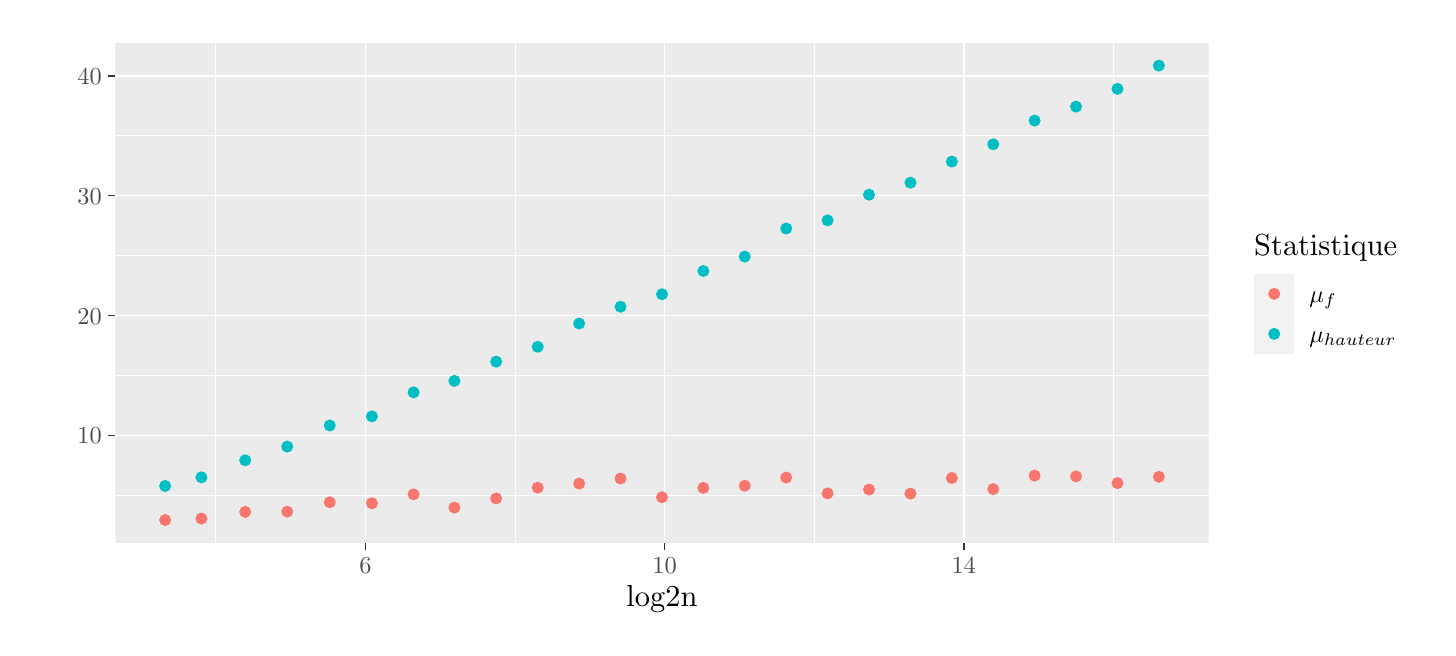
\begin{tikzpicture}[x=1pt,y=1pt]
\definecolor{fillColor}{RGB}{255,255,255}
\path[use as bounding box,fill=fillColor,fill opacity=0.00] (0,0) rectangle (505.89,216.81);
\begin{scope}
\path[clip] (  0.00,  0.00) rectangle (505.89,216.81);
\definecolor{drawColor}{RGB}{255,255,255}
\definecolor{fillColor}{RGB}{255,255,255}

\path[draw=drawColor,line width= 0.6pt,line join=round,line cap=round,fill=fillColor] (  0.00,  0.00) rectangle (505.89,216.81);
\end{scope}
\begin{scope}
\path[clip] ( 31.71, 30.69) rectangle (426.70,211.31);
\definecolor{fillColor}{gray}{0.92}

\path[fill=fillColor] ( 31.71, 30.69) rectangle (426.70,211.31);
\definecolor{drawColor}{RGB}{255,255,255}

\path[draw=drawColor,line width= 0.3pt,line join=round] ( 31.71, 47.74) --
	(426.70, 47.74);

\path[draw=drawColor,line width= 0.3pt,line join=round] ( 31.71, 91.09) --
	(426.70, 91.09);

\path[draw=drawColor,line width= 0.3pt,line join=round] ( 31.71,134.44) --
	(426.70,134.44);

\path[draw=drawColor,line width= 0.3pt,line join=round] ( 31.71,177.78) --
	(426.70,177.78);

\path[draw=drawColor,line width= 0.3pt,line join=round] ( 67.99, 30.69) --
	( 67.99,211.31);

\path[draw=drawColor,line width= 0.3pt,line join=round] (176.08, 30.69) --
	(176.08,211.31);

\path[draw=drawColor,line width= 0.3pt,line join=round] (284.18, 30.69) --
	(284.18,211.31);

\path[draw=drawColor,line width= 0.3pt,line join=round] (392.27, 30.69) --
	(392.27,211.31);

\path[draw=drawColor,line width= 0.6pt,line join=round] ( 31.71, 69.41) --
	(426.70, 69.41);

\path[draw=drawColor,line width= 0.6pt,line join=round] ( 31.71,112.76) --
	(426.70,112.76);

\path[draw=drawColor,line width= 0.6pt,line join=round] ( 31.71,156.11) --
	(426.70,156.11);

\path[draw=drawColor,line width= 0.6pt,line join=round] ( 31.71,199.46) --
	(426.70,199.46);

\path[draw=drawColor,line width= 0.6pt,line join=round] (122.04, 30.69) --
	(122.04,211.31);

\path[draw=drawColor,line width= 0.6pt,line join=round] (230.13, 30.69) --
	(230.13,211.31);

\path[draw=drawColor,line width= 0.6pt,line join=round] (338.23, 30.69) --
	(338.23,211.31);
\definecolor{drawColor}{RGB}{0,191,196}
\definecolor{fillColor}{RGB}{0,191,196}

\path[draw=drawColor,line width= 0.4pt,line join=round,line cap=round,fill=fillColor] ( 49.67, 51.21) circle (  1.96);
\definecolor{drawColor}{RGB}{248,118,109}
\definecolor{fillColor}{RGB}{248,118,109}

\path[draw=drawColor,line width= 0.4pt,line join=round,line cap=round,fill=fillColor] ( 49.67, 38.90) circle (  1.96);
\definecolor{drawColor}{RGB}{0,191,196}
\definecolor{fillColor}{RGB}{0,191,196}

\path[draw=drawColor,line width= 0.4pt,line join=round,line cap=round,fill=fillColor] ( 62.78, 54.33) circle (  1.96);
\definecolor{drawColor}{RGB}{248,118,109}
\definecolor{fillColor}{RGB}{248,118,109}

\path[draw=drawColor,line width= 0.4pt,line join=round,line cap=round,fill=fillColor] ( 62.78, 39.42) circle (  1.96);
\definecolor{drawColor}{RGB}{0,191,196}
\definecolor{fillColor}{RGB}{0,191,196}

\path[draw=drawColor,line width= 0.4pt,line join=round,line cap=round,fill=fillColor] ( 78.59, 60.48) circle (  1.96);
\definecolor{drawColor}{RGB}{248,118,109}
\definecolor{fillColor}{RGB}{248,118,109}

\path[draw=drawColor,line width= 0.4pt,line join=round,line cap=round,fill=fillColor] ( 78.59, 41.84) circle (  1.96);
\definecolor{drawColor}{RGB}{0,191,196}
\definecolor{fillColor}{RGB}{0,191,196}

\path[draw=drawColor,line width= 0.4pt,line join=round,line cap=round,fill=fillColor] ( 93.78, 65.43) circle (  1.96);
\definecolor{drawColor}{RGB}{248,118,109}
\definecolor{fillColor}{RGB}{248,118,109}

\path[draw=drawColor,line width= 0.4pt,line join=round,line cap=round,fill=fillColor] ( 93.78, 41.93) circle (  1.96);
\definecolor{drawColor}{RGB}{0,191,196}
\definecolor{fillColor}{RGB}{0,191,196}

\path[draw=drawColor,line width= 0.4pt,line join=round,line cap=round,fill=fillColor] (109.16, 73.05) circle (  1.96);
\definecolor{drawColor}{RGB}{248,118,109}
\definecolor{fillColor}{RGB}{248,118,109}

\path[draw=drawColor,line width= 0.4pt,line join=round,line cap=round,fill=fillColor] (109.16, 45.31) circle (  1.96);
\definecolor{drawColor}{RGB}{0,191,196}
\definecolor{fillColor}{RGB}{0,191,196}

\path[draw=drawColor,line width= 0.4pt,line join=round,line cap=round,fill=fillColor] (124.40, 76.35) circle (  1.96);
\definecolor{drawColor}{RGB}{248,118,109}
\definecolor{fillColor}{RGB}{248,118,109}

\path[draw=drawColor,line width= 0.4pt,line join=round,line cap=round,fill=fillColor] (124.40, 44.96) circle (  1.96);
\definecolor{drawColor}{RGB}{0,191,196}
\definecolor{fillColor}{RGB}{0,191,196}

\path[draw=drawColor,line width= 0.4pt,line join=round,line cap=round,fill=fillColor] (139.44, 85.02) circle (  1.96);
\definecolor{drawColor}{RGB}{248,118,109}
\definecolor{fillColor}{RGB}{248,118,109}

\path[draw=drawColor,line width= 0.4pt,line join=round,line cap=round,fill=fillColor] (139.44, 48.17) circle (  1.96);
\definecolor{drawColor}{RGB}{0,191,196}
\definecolor{fillColor}{RGB}{0,191,196}

\path[draw=drawColor,line width= 0.4pt,line join=round,line cap=round,fill=fillColor] (154.19, 89.18) circle (  1.96);
\definecolor{drawColor}{RGB}{248,118,109}
\definecolor{fillColor}{RGB}{248,118,109}

\path[draw=drawColor,line width= 0.4pt,line join=round,line cap=round,fill=fillColor] (154.19, 43.40) circle (  1.96);
\definecolor{drawColor}{RGB}{0,191,196}
\definecolor{fillColor}{RGB}{0,191,196}

\path[draw=drawColor,line width= 0.4pt,line join=round,line cap=round,fill=fillColor] (169.28, 96.12) circle (  1.96);
\definecolor{drawColor}{RGB}{248,118,109}
\definecolor{fillColor}{RGB}{248,118,109}

\path[draw=drawColor,line width= 0.4pt,line join=round,line cap=round,fill=fillColor] (169.28, 46.70) circle (  1.96);
\definecolor{drawColor}{RGB}{0,191,196}
\definecolor{fillColor}{RGB}{0,191,196}

\path[draw=drawColor,line width= 0.4pt,line join=round,line cap=round,fill=fillColor] (184.29,101.49) circle (  1.96);
\definecolor{drawColor}{RGB}{248,118,109}
\definecolor{fillColor}{RGB}{248,118,109}

\path[draw=drawColor,line width= 0.4pt,line join=round,line cap=round,fill=fillColor] (184.29, 50.60) circle (  1.96);
\definecolor{drawColor}{RGB}{0,191,196}
\definecolor{fillColor}{RGB}{0,191,196}

\path[draw=drawColor,line width= 0.4pt,line join=round,line cap=round,fill=fillColor] (199.27,109.90) circle (  1.96);
\definecolor{drawColor}{RGB}{248,118,109}
\definecolor{fillColor}{RGB}{248,118,109}

\path[draw=drawColor,line width= 0.4pt,line join=round,line cap=round,fill=fillColor] (199.27, 52.07) circle (  1.96);
\definecolor{drawColor}{RGB}{0,191,196}
\definecolor{fillColor}{RGB}{0,191,196}

\path[draw=drawColor,line width= 0.4pt,line join=round,line cap=round,fill=fillColor] (214.23,115.97) circle (  1.96);
\definecolor{drawColor}{RGB}{248,118,109}
\definecolor{fillColor}{RGB}{248,118,109}

\path[draw=drawColor,line width= 0.4pt,line join=round,line cap=round,fill=fillColor] (214.23, 53.89) circle (  1.96);
\definecolor{drawColor}{RGB}{0,191,196}
\definecolor{fillColor}{RGB}{0,191,196}

\path[draw=drawColor,line width= 0.4pt,line join=round,line cap=round,fill=fillColor] (229.21,120.48) circle (  1.96);
\definecolor{drawColor}{RGB}{248,118,109}
\definecolor{fillColor}{RGB}{248,118,109}

\path[draw=drawColor,line width= 0.4pt,line join=round,line cap=round,fill=fillColor] (229.21, 47.13) circle (  1.96);
\definecolor{drawColor}{RGB}{0,191,196}
\definecolor{fillColor}{RGB}{0,191,196}

\path[draw=drawColor,line width= 0.4pt,line join=round,line cap=round,fill=fillColor] (244.15,128.89) circle (  1.96);
\definecolor{drawColor}{RGB}{248,118,109}
\definecolor{fillColor}{RGB}{248,118,109}

\path[draw=drawColor,line width= 0.4pt,line join=round,line cap=round,fill=fillColor] (244.15, 50.51) circle (  1.96);
\definecolor{drawColor}{RGB}{0,191,196}
\definecolor{fillColor}{RGB}{0,191,196}

\path[draw=drawColor,line width= 0.4pt,line join=round,line cap=round,fill=fillColor] (259.12,134.09) circle (  1.96);
\definecolor{drawColor}{RGB}{248,118,109}
\definecolor{fillColor}{RGB}{248,118,109}

\path[draw=drawColor,line width= 0.4pt,line join=round,line cap=round,fill=fillColor] (259.12, 51.29) circle (  1.96);
\definecolor{drawColor}{RGB}{0,191,196}
\definecolor{fillColor}{RGB}{0,191,196}

\path[draw=drawColor,line width= 0.4pt,line join=round,line cap=round,fill=fillColor] (274.09,144.23) circle (  1.96);
\definecolor{drawColor}{RGB}{248,118,109}
\definecolor{fillColor}{RGB}{248,118,109}

\path[draw=drawColor,line width= 0.4pt,line join=round,line cap=round,fill=fillColor] (274.09, 54.24) circle (  1.96);
\definecolor{drawColor}{RGB}{0,191,196}
\definecolor{fillColor}{RGB}{0,191,196}

\path[draw=drawColor,line width= 0.4pt,line join=round,line cap=round,fill=fillColor] (289.05,147.18) circle (  1.96);
\definecolor{drawColor}{RGB}{248,118,109}
\definecolor{fillColor}{RGB}{248,118,109}

\path[draw=drawColor,line width= 0.4pt,line join=round,line cap=round,fill=fillColor] (289.05, 48.52) circle (  1.96);
\definecolor{drawColor}{RGB}{0,191,196}
\definecolor{fillColor}{RGB}{0,191,196}

\path[draw=drawColor,line width= 0.4pt,line join=round,line cap=round,fill=fillColor] (304.01,156.46) circle (  1.96);
\definecolor{drawColor}{RGB}{248,118,109}
\definecolor{fillColor}{RGB}{248,118,109}

\path[draw=drawColor,line width= 0.4pt,line join=round,line cap=round,fill=fillColor] (304.01, 49.91) circle (  1.96);
\definecolor{drawColor}{RGB}{0,191,196}
\definecolor{fillColor}{RGB}{0,191,196}

\path[draw=drawColor,line width= 0.4pt,line join=round,line cap=round,fill=fillColor] (318.98,160.79) circle (  1.96);
\definecolor{drawColor}{RGB}{248,118,109}
\definecolor{fillColor}{RGB}{248,118,109}

\path[draw=drawColor,line width= 0.4pt,line join=round,line cap=round,fill=fillColor] (318.98, 48.43) circle (  1.96);
\definecolor{drawColor}{RGB}{0,191,196}
\definecolor{fillColor}{RGB}{0,191,196}

\path[draw=drawColor,line width= 0.4pt,line join=round,line cap=round,fill=fillColor] (333.94,168.42) circle (  1.96);
\definecolor{drawColor}{RGB}{248,118,109}
\definecolor{fillColor}{RGB}{248,118,109}

\path[draw=drawColor,line width= 0.4pt,line join=round,line cap=round,fill=fillColor] (333.94, 54.07) circle (  1.96);
\definecolor{drawColor}{RGB}{0,191,196}
\definecolor{fillColor}{RGB}{0,191,196}

\path[draw=drawColor,line width= 0.4pt,line join=round,line cap=round,fill=fillColor] (348.90,174.66) circle (  1.96);
\definecolor{drawColor}{RGB}{248,118,109}
\definecolor{fillColor}{RGB}{248,118,109}

\path[draw=drawColor,line width= 0.4pt,line join=round,line cap=round,fill=fillColor] (348.90, 50.08) circle (  1.96);
\definecolor{drawColor}{RGB}{0,191,196}
\definecolor{fillColor}{RGB}{0,191,196}

\path[draw=drawColor,line width= 0.4pt,line join=round,line cap=round,fill=fillColor] (363.86,183.25) circle (  1.96);
\definecolor{drawColor}{RGB}{248,118,109}
\definecolor{fillColor}{RGB}{248,118,109}

\path[draw=drawColor,line width= 0.4pt,line join=round,line cap=round,fill=fillColor] (363.86, 54.93) circle (  1.96);
\definecolor{drawColor}{RGB}{0,191,196}
\definecolor{fillColor}{RGB}{0,191,196}

\path[draw=drawColor,line width= 0.4pt,line join=round,line cap=round,fill=fillColor] (378.82,188.27) circle (  1.96);
\definecolor{drawColor}{RGB}{248,118,109}
\definecolor{fillColor}{RGB}{248,118,109}

\path[draw=drawColor,line width= 0.4pt,line join=round,line cap=round,fill=fillColor] (378.82, 54.67) circle (  1.96);
\definecolor{drawColor}{RGB}{0,191,196}
\definecolor{fillColor}{RGB}{0,191,196}

\path[draw=drawColor,line width= 0.4pt,line join=round,line cap=round,fill=fillColor] (393.79,194.69) circle (  1.96);
\definecolor{drawColor}{RGB}{248,118,109}
\definecolor{fillColor}{RGB}{248,118,109}

\path[draw=drawColor,line width= 0.4pt,line join=round,line cap=round,fill=fillColor] (393.79, 52.25) circle (  1.96);
\definecolor{drawColor}{RGB}{0,191,196}
\definecolor{fillColor}{RGB}{0,191,196}

\path[draw=drawColor,line width= 0.4pt,line join=round,line cap=round,fill=fillColor] (408.75,203.10) circle (  1.96);
\definecolor{drawColor}{RGB}{248,118,109}
\definecolor{fillColor}{RGB}{248,118,109}

\path[draw=drawColor,line width= 0.4pt,line join=round,line cap=round,fill=fillColor] (408.75, 54.50) circle (  1.96);
\end{scope}
\begin{scope}
\path[clip] (  0.00,  0.00) rectangle (505.89,216.81);
\definecolor{drawColor}{gray}{0.30}

\node[text=drawColor,anchor=base east,inner sep=0pt, outer sep=0pt, scale=  0.88] at ( 26.76, 66.38) {10};

\node[text=drawColor,anchor=base east,inner sep=0pt, outer sep=0pt, scale=  0.88] at ( 26.76,109.73) {20};

\node[text=drawColor,anchor=base east,inner sep=0pt, outer sep=0pt, scale=  0.88] at ( 26.76,153.08) {30};

\node[text=drawColor,anchor=base east,inner sep=0pt, outer sep=0pt, scale=  0.88] at ( 26.76,196.43) {40};
\end{scope}
\begin{scope}
\path[clip] (  0.00,  0.00) rectangle (505.89,216.81);
\definecolor{drawColor}{gray}{0.20}

\path[draw=drawColor,line width= 0.6pt,line join=round] ( 28.96, 69.41) --
	( 31.71, 69.41);

\path[draw=drawColor,line width= 0.6pt,line join=round] ( 28.96,112.76) --
	( 31.71,112.76);

\path[draw=drawColor,line width= 0.6pt,line join=round] ( 28.96,156.11) --
	( 31.71,156.11);

\path[draw=drawColor,line width= 0.6pt,line join=round] ( 28.96,199.46) --
	( 31.71,199.46);
\end{scope}
\begin{scope}
\path[clip] (  0.00,  0.00) rectangle (505.89,216.81);
\definecolor{drawColor}{gray}{0.20}

\path[draw=drawColor,line width= 0.6pt,line join=round] (122.04, 27.94) --
	(122.04, 30.69);

\path[draw=drawColor,line width= 0.6pt,line join=round] (230.13, 27.94) --
	(230.13, 30.69);

\path[draw=drawColor,line width= 0.6pt,line join=round] (338.23, 27.94) --
	(338.23, 30.69);
\end{scope}
\begin{scope}
\path[clip] (  0.00,  0.00) rectangle (505.89,216.81);
\definecolor{drawColor}{gray}{0.30}

\node[text=drawColor,anchor=base,inner sep=0pt, outer sep=0pt, scale=  0.88] at (122.04, 19.68) {6};

\node[text=drawColor,anchor=base,inner sep=0pt, outer sep=0pt, scale=  0.88] at (230.13, 19.68) {10};

\node[text=drawColor,anchor=base,inner sep=0pt, outer sep=0pt, scale=  0.88] at (338.23, 19.68) {14};
\end{scope}
\begin{scope}
\path[clip] (  0.00,  0.00) rectangle (505.89,216.81);
\definecolor{drawColor}{RGB}{0,0,0}

\node[text=drawColor,anchor=base,inner sep=0pt, outer sep=0pt, scale=  1.10] at (229.21,  7.64) {log2n};
\end{scope}
\begin{scope}
\path[clip] (  0.00,  0.00) rectangle (505.89,216.81);
\definecolor{fillColor}{RGB}{255,255,255}

\path[fill=fillColor] (437.70, 93.44) rectangle (500.39,148.56);
\end{scope}
\begin{scope}
\path[clip] (  0.00,  0.00) rectangle (505.89,216.81);
\definecolor{drawColor}{RGB}{0,0,0}

\node[text=drawColor,anchor=base west,inner sep=0pt, outer sep=0pt, scale=  1.10] at (443.20,134.41) {Statistique};
\end{scope}
\begin{scope}
\path[clip] (  0.00,  0.00) rectangle (505.89,216.81);
\definecolor{fillColor}{gray}{0.95}

\path[fill=fillColor] (443.20,113.39) rectangle (457.66,127.84);
\end{scope}
\begin{scope}
\path[clip] (  0.00,  0.00) rectangle (505.89,216.81);
\definecolor{drawColor}{RGB}{248,118,109}
\definecolor{fillColor}{RGB}{248,118,109}

\path[draw=drawColor,line width= 0.4pt,line join=round,line cap=round,fill=fillColor] (450.43,120.62) circle (  1.96);
\end{scope}
\begin{scope}
\path[clip] (  0.00,  0.00) rectangle (505.89,216.81);
\definecolor{fillColor}{gray}{0.95}

\path[fill=fillColor] (443.20, 98.94) rectangle (457.66,113.39);
\end{scope}
\begin{scope}
\path[clip] (  0.00,  0.00) rectangle (505.89,216.81);
\definecolor{drawColor}{RGB}{0,191,196}
\definecolor{fillColor}{RGB}{0,191,196}

\path[draw=drawColor,line width= 0.4pt,line join=round,line cap=round,fill=fillColor] (450.43,106.16) circle (  1.96);
\end{scope}
\begin{scope}
\path[clip] (  0.00,  0.00) rectangle (505.89,216.81);
\definecolor{drawColor}{RGB}{0,0,0}

\node[text=drawColor,anchor=base west,inner sep=0pt, outer sep=0pt, scale=  0.88] at (463.16,117.59) {$\mu_f$};
\end{scope}
\begin{scope}
\path[clip] (  0.00,  0.00) rectangle (505.89,216.81);
\definecolor{drawColor}{RGB}{0,0,0}

\node[text=drawColor,anchor=base west,inner sep=0pt, outer sep=0pt, scale=  0.88] at (463.16,103.13) {$\mu_{hauteur}$};
\end{scope}
\end{tikzpicture}

    \vspace{-1cm}
    \caption{Les variations du moyen facteur de déséquilibre et moyen hauteur par rapport à $\log_2 n$. Il est évident qu'il y a une corresponance linéaire entre nos statistiques observés et on peut constater que $\mu_f,\ \mu_{hauteur} \in \Theta(\log_2 n)$. }
\end{figure}

\vspace{1cm}
\noindent \asgold{Remarques :}

Le code source de ce document se trouve sur le github dans le répertoire \texttt{tex/}. Le binaire \texttt{bst} compilé pour x86-64 est inclu dans le zip rendu sur moodle. Sinon, vous pouvez téléchargé le projet
et suivre les instructions du \texttt{README.md} pour construire le projet tp3.

% \newpage
\end{document}